\chapter{Integration Into Machine Translation Systems}
\label{chap:integration}
In this chapter, we demonstrate how our CL-WSD techniques can be integrated
into running machine translation systems, with the goal of improving lexical
selection in practice, while minimizing code changes to the MT software. We
translate from Spanish to Guarani with Moses\cite{koehn-EtAl:2007:PosterDemo},
an off-the-shelf phrase-based statistical MT system, and from Spanish to
Quechua with SQUOIA, a rule-based MT system that was developed by Rios \emph{et
al.} at the University of Zürich. These two integrations are meant to be simple
proofs of concept, rather than an attempt to define a best practice, but they
demonstrate at least conceptually how CL-WSD can be used with these translation
systems.  Afterwards, we look at evaluating Chipa's effect on MT output in both
of these use cases.

Among other pieces of software related to this work, especially the corpus
preparation scripts, the code to integrate Chipa into these machine
translation systems is in a package called Tereré \footnote{Available at
\url{http://github.com/alexrudnick/terere} ; Tereré is a cold variety of yerba
mate brewed with ice water; it is a specifically Paraguayan specialty.}.



%% XXX working here
Lexical ambiguity is a significant problem facing rule-based machine
translation systems (CITATION NEEDED), as many words have several possible
translations in a given target language, each of which can be considered a
sense of the word from the source language.

The difficulty of resolving these ambiguities is mitigated for 
statistical machine translation systems for language pairs with large bilingual
corpora, as large n-gram language models and phrase tables containing common
multi-word expressions can encourage coherent word choices.
For most language pairs these resources are not available, so a primarily
rule-based approach becomes attractive.

In cases where some training data is available, though, we can
investigate hybrid RBMT and machine learning approaches, leveraging small and
potentially growing bilingual corpora.

... show how it allows us to learn from the available bitext to
make better lexical choices, with very few code changes to the base system.
The integration enables SQUOIA to take advantage of any available bitext
without significantly changing its design, and to improve its word choices as
additional bitext becomes available.

While there are some rules for lexical selection, they have been written by
hand and only cover a small subset of the vocabulary in a limited number of
contexts.
In this work, we supplement these rules with classifiers learned from
Spanish-Quechua bitext.
These classifiers make use of regularities that may not be obvious to human
rule-writers, providing improved lexical selection for any word type that has
adequate coverage in the training corpus.





\section{Integrating Chipa into Phrase-Based Statistical Machine Translation}
Moses\footnote{Available at
\url{http://statmt.org/moses/}} is a mature,
well-maintained and popular statistical machine translation package, in broad
use for both research and practical purposes. Conveniently for our work here,
it includes an interface for adding feature functions\footnote{See
\url{http://www.statmt.org/moses/?n=Moses.FeatureFunctions} for documentation.}
to guide its decoding process.

Moses, like many SMT systems, combines signals from different subcomponents
when searching through the space of possible translations. It does this using a
log-linear model, in which each component scores a candidate translation, and
then the scores from the different components are combined with a weighted sum.
Some typical components are the probabilities learned for a given phrase during
phrase extraction (without regard to context) in both translation directions,
scores from the target-language language model, learned distortion models that
reflect estimated differences in word order between source and target
languages, and a handful of other features\footnote{For an overview of
techniques commonly used in phrase-based statistical MT, please see Koehn's
book on the subject \cite{koehn2010statistical}.}. The weights for each
subcomponent are typically tuned with Minimum Error-Rate Training, or ``MERT"
\cite{och:2003:ACL}.

Scores in this framework are expected to represent log probabilities, meaning
that, concretely, they are real numbers less than 0, as the logarithm of a
number between 0 and 1 will be negative. The beam search procedure then
attempts to maximize the total score for a translation, which means finding a
translation with a score as high as possible, \emph{i.e.}, maximally close to
0.

We built a simple phrase-based SMT system with Moses and used this feature
function API to have Chipa evaluate candidate translations.
For simplicity, we added a constraint in the Moses phrase-extraction system
so that the source side of all phrases must be at most one token long, to match
the alignments used in the previous chapters.

During the search through the space of possible translations, Moses proposes
candidate translations for each source word to Chipa ...
which provides a score based on how likely the translation seems to the CL-WSD
system, based on the entire source-language sentence context. This score is
returned to Moses, which combines all of the available features in a log-linear
combination.

The weights for all of the features provided to the system (translation
probabilities, LM scores, CL-WSD scores, and perhaps others) can be tuned on a
development set with MERT \cite{och:2003:ACL}; thus, if CL-WSD scores turn out
to be useful for achieving high BLEU scores on the development set sentences,
Chipa's feature function will be assigned a higher weight. If not, its advice
carries less weight, than, for example, that of the language model.


\subsection{Interfacing between Moses and Chipa}
%% write about how we can't we just annotate the phrase table for individual
%% sentences just before decoding -- we need to know about the phrase *in a
%% context* and that's the point.
We implemented a simple protocol for communication between the Moses C++ code
and the Chipa server, based on Unix pipes; see Figure
\ref{fig:moses-chipa-diagram} for a visual aid. In earlier work with SQUOIA
\cite{rudnick:saltmil2014}, we had communicated between Chipa and the machine
translation system with XML-RPC \footnote{\url{http://xmlrpc.scripting.com/}},
but for simplicity of implementation, we built a simpler text-based protocol.

Named Unix pipes, or FIFOs, allow the creation of a special kind of filesystem
object whereby messages can be passed between processes in the same computer.
Here Moses requests an evaluation for a certain translation of a
source-language phrase, and Chipa returns a score based on how likely it
considers that phrase, represented as log probabilities. 

\begin{figure}
  \begin{centering}
  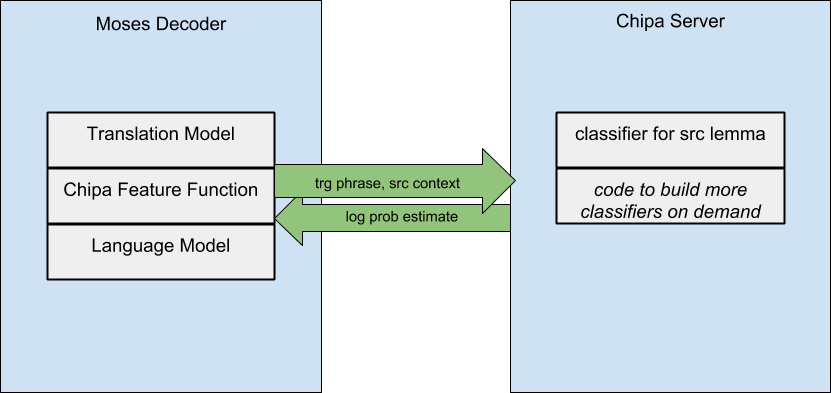
\includegraphics[width=15cm]{moses-chipa-diagram.png}
  \end{centering}
  \caption{Schematic diagram showing the relationship between the Moses decoder
  process, running the custom-made Chipa feature function, which communicates
  with the Chipa server process. The Chipa server returns probability
  estimates for proposed target-language phrases based on the given
  source-sentence context, when available.}
  \label{fig:moses-chipa-diagram}
\end{figure}

\section{Integrating Chipa into Rule-Based Machine Translation}


\subsection{The SQUOIA RBMT system}
SQUOIA\footnote{Code available at \url{https://github.com/a-rios/squoia} ;
the project is more broadly described at
\url{https://www.cl.uzh.ch/en/research/machine-translation/hybridmt.html}}
is a system for machine translation, primarily from Spanish to the Cuzco
dialect of Quechua, spoken around the Peruvian city of Cuzco.

SQUOIA was developed by a team at the University of Zurich. For the most
part, it is a classical rule-based system, although the team has
developed techniques for predicting verb morphology with machine
learning methods, in cases when its rules cannot reliably disambiguate
\cite{riosgonzales-gohring:2013:HyTra}. It does not, by default, use machine
learning for lexical selection as such,
although it does include a language model to help select among the
translations licensed by its transfer rules, and the initial input analysis
stages use open-source NLP tools based on learned models. SQUOIA uses
FreeLing \cite{padro12} for morphological analysis and named-entity
recognition, Wapiti \cite{lavergne2010practical} for tagging, and DeSr
\cite{attardi-EtAl:2007:EMNLP-CoNLL2007} for parsing.

SQUOIA's architecture is based on the Matxin system \cite{matxin2005}, which
was originally intended for translating from Spanish to Basque. It consists of
a pipeline of smaller steps, each of which passes along a tree describing the
current input text and transformations that have been applied to it, in XML
form. As the steps progress, the input Spanish is analyzed and gradually
transformed into Quechua output. Many modules focus on very particular parts of
the representation, leaving most of their input unchanged; for example, one
phase performs coreference resolution, and another phase uses rules to try to
decide whether an instance of the Spanish preposition \emph{de} should be
translated into Quechua as indicating the ablative case (direction of motion),
or the genitive case (posession). Please see Figure \ref{fig:squoia-steps} for
an overview of the most important steps in the SQUOIA pipeline.

%% XXX working here

In order to add Chipa CL-WSD to SQUOIA, we added an additional intermediate
step to the pipeline that reads the XML representation of the input sentences,
finds lexical-selection ambiguities that we can attempt to resolve with Chipa,
constrains those choices lexical choices based on the recommendations of our
classifiers, and then passes these choices to subsequent steps.

\begin{figure}
  \begin{itemize}
  \item Tokenization, morphological analysis, tagging, parsing.
  \item Disambiguating Spanish verbs with rules that match on contextual clues
  (low recall; the rules are manually crafted by linguists)
  \item Disambiguating Spanish verbs with an SVM classifier.
  \item Lexical lookup and transfer: insert all possible translations for every
  input token from the bilingual dictionary.
  \item Rule-based disambiguation, attempting to eliminate possible
  lexical-selection ambiguities and morphological choices. (similarly low
  coverage; it is not feasible for linguists to write rules for all possible
  contexts for every word type in the lexicon)
  \item \emph{DISAMBIGUATION WITH CHIPA INSERTED HERE}
  \item Syntactic transfer, building more Quechua-like syntactic structures
  (rule-based).
  \item Reordering based on new syntactic trees (rule-based).
  \item Use KenLM language models trained over Quechua words and morphemes to
  choose most likely alternatives remaining.
  \item Morphological generation: produce Quechua surface forms with a finite
  state transducer, output n-best list.
  \end{itemize}

  \caption{An overview of the steps in the SQUOIA MT system; there are a few
  more, handling specific circumstances and parts of speech.}
  \label{fig:squoia-steps}
\end{figure}

%% XXX: working here what's with all this text

In its current design, SQUOIA makes word choices based on its bilingual
lexicon; the possible translations for a given word or multi-word expression
are retrieved from a dictionary on demand.

The rest of the system makes use of a classical transfer procedure.
A following
module moves syntactic information between the nodes and the chunks in the
tree, and finally, the tree is reordered according to the basic word order in
the target language.

%% XXX: working here
In order to integrate Chipa into SQUOIA, we added an additional lexical
selection stage to the SQUOIA pipeline, occurring after the rule-based
disambiguation modules, but before a number of other steps. This new module
examines the XML tree structure of a SQUOIA translation in progress, and finds
nodes in the tree where there are several possible Quechua lemmas that may be
chosen as a translation. It then extracts the surface forms and lemmas of the
input sentence from the current XML tree structure, and passes these along to
the Chipa system so that we can make a prediction as to what the correct
translation for that input token should be.

For each word with such multiple translation possibilities, we look at each of
the translations under consideration by SQUOIA, and if any of them was the top 
classification output from the Chipa classifiers, we constrain SQUOIA to take
that choice by removing the other available options.

If there are no such overlapping translations, we make no changes to the input
tree, and allow SQUOIA to proceed as normal. Notably, since Chipa and SQUOIA
do not share the same lexicon and bitext alignments may be noisy, translations
observed in the bitext may be unknown to the SQUOIA system, and lexical entries
in the SQUOIA dictionary may not be attested in the training data.


\section{Translation Evaluation for Spanish-Guarani}

%% TODO: explain how we sampled test sets, what it means that we picked verses
%% rather than sentences

\subsection{Results: BLEU scores for Spanish-Guarani}

In Figure \ref{fig:bleu-es-gn}, we report BLEU scores for our PBMT system with
Chipa enabled.
%% TODO Explain what's up with training with MERT and then turning off that
%% feature.

\begin{figure*}
  \begin{centering}
  \begin{tabulary}{\textwidth}{|R|L|}
    \hline
    setting & BLEU \\
    \hline
    Moses with Chipa enabled &  16.24 \\
    \hline
    Same system, with Chipa disabled &  10.01 \\
    \hline
  \end{tabulary}
  \end{centering}
  \caption{BLEU scores on our Spanish-Guarani test set. Note that this is
  translating to \emph{lemmatized} Guarani, rather than having to predict
  fully-inflected forms.}
  \label{fig:bleu-es-gn}
\end{figure*}


\section{Translation Evaluation for Spanish-Quechua}

In order to evaluate the effect of Chipa on lexical selection in a live
translation task, we used SQUOIA to translate a hundred verses sampled from our
Spanish-Quechua Bible bitext, both in its default settings, and with the
addition of Chipa. The BLEU scores for SQUOIA output on this test set were
quite low (lower than one BLEU point), and were not improved by adding the
Chipa CL-WSD, but this is a rather more difficult task, since we are attempting
to generate fully-inflected Quechua surface forms, rather than selecting
appropriate lemmas.

In any case, here we will show examples of word choices that were changed with
the addition of Chipa CL-WSD, and, armed with our Spanish-Quechua dictionary
\cite{academiamayor}, determine whether they are more or less appropriate than
the choices that the SQUOIA system would have made on its own. For some
examples chosen from the sampled test set, see Figure
\ref{fig:some-spanish-verses-with-changes}. 

One pattern that we find among the changed output is that Chipa tends to
encourage SQUOIA to choose \emph{churi} (a son, when discussed with regard to
his father) rather than the more generic \emph{wawa}, which can refer to any
child; for most of the test sentences where we saw this change happen, it
seemed like an appropriate choice. For example, in Sentence
\ref{sent:putyourhand}, we are referring to a son of a particular man, so this
seems like a good choice.

We see when translating Sentence \ref{sent:alreadydead}  from Spanish to
Quechua, without Chipa, SQUOIA translates \emph{llamando} ('calling') to
\emph{sutikuspa}, where \emph{suti} is the sense of ``llamar" that refers to
naming. However, with Chipa, SQUOIA picks \emph{waqyaspa}, where \emph{waqyay}
is the communicative sense, rather than the naming sense.

Many changes caused by Chipa seem to be different choices among near synonyms.
For example, in Sentence \ref{sent:burning}, without Chipa, we translate
\emph{ardiente} as \emph{k'anaq}, which seems to be a good translation, meaning
``glowing, ardently burning". With Chipa, it becomes \emph{'yawraq'} 'burning,
glowing'. And one difference revealed an ambiguity in Spanish that is clearly
distinguished in Quechua: in Sentence \ref{sent:reins}, without Chipa, we
translate \emph{labios} 'lips' as an inflection of \emph{wirp'a}, which
apparently only refers to the lower lip; with Chipa, we choose an inflection of
\emph{sirphi}, which seems to refer to only the upper lip
\footnote{Also, more modern English translations seem to choose something like
``innermost being" rather than referring to one's innards, but the King James
Version uses the term ``reins", which apparently historically referred to the
kidneys.}.

We note in Sentence \ref{sent:llama} a serious word-sense issue that Chipa did
not manage to fix; in both cases, SQUOIA failed to interpret \emph{llama} as
'flame'\footnote{The Spanish token \emph{llama} can be an inflection of the
verb \emph{llamar} 'to call', or as a noun, 'flame', or of course it can refer
to llama the animal, which is a loan word from Quechua.}; this seems to be a
cascading error from part-of-speech tagging, as SQUOIA's bundled tagger marked
it as a verb. In any case, without SQUOIA, we choose an inflection of
\emph{waqya}, which is the 'call out' sense of \emph{llamar}, and with Chipa,
we choose an inflection of \emph{suti}, the 'naming' sense. Neither of these
are correct.

\begin{figure*}
\enumsentence{
Jehová dijo a Moisés: -- Toma a Josué hijo de Nun, hombre en el cual hay
espíritu, y pon tu mano sobre él. \emph{``Jehovah said to Moses: - Take Joshua
son of Nun, man in whom there is spirit, and put your hand on him.", Numbers
27:18}}
\label{sent:putyourhand}

\enumsentence{
Pilato se sorprendió de que ya hubiera muerto, y llamando al centurión, le
preguntó si ya estaba muerto. \emph{``Pilate was surprised to hear that he had
already died, and calling the centurion, asked him if he was already dead.",
Mark 15:44}}
\label{sent:alreadydead}

\enumsentence{
Y cualquiera que no se postre y adore, inmediatamente será echado dentro de un
horno de fuego ardiente. \emph{``And whoever does not fall down and worship
will immediately be thrown into a blazing furnace.", Daniel 3:6}}
\label{sent:burning}

\enumsentence{
Y mis entrañas también se alegrarán cuando tus labios hablen con rectitud. \emph{Proverbs 23:16}}
\label{sent:reins}

\enumsentence{
Por tanto, como la lengua del fuego consume el rastrojo y la llama devora la
paja, así será su raíz como podredumbre y su flor se desvanecerá como polvo,
porque desecharon la ley de Jehová de los ejércitos y abominaron la palabra del
Santo de Israel. \emph{Isaiah 5:24}}
\label{sent:llama}
  \caption{Selected Spanish passages for which adding Chipa generated different
  Quechua translations.}
  \label{fig:some-spanish-verses-with-changes}
\end{figure*}

\section{Discussion}
